
\section{Results}


\subsection{Effect of spatial structure in PD and HD games}
In our first simulation experiment, we compared the effect of spatial structure on the persistence of cooperators in the PD and HD games.


(figure \ref{fig: task1_4plot})



\begin{figure}[H]
	\centering 
	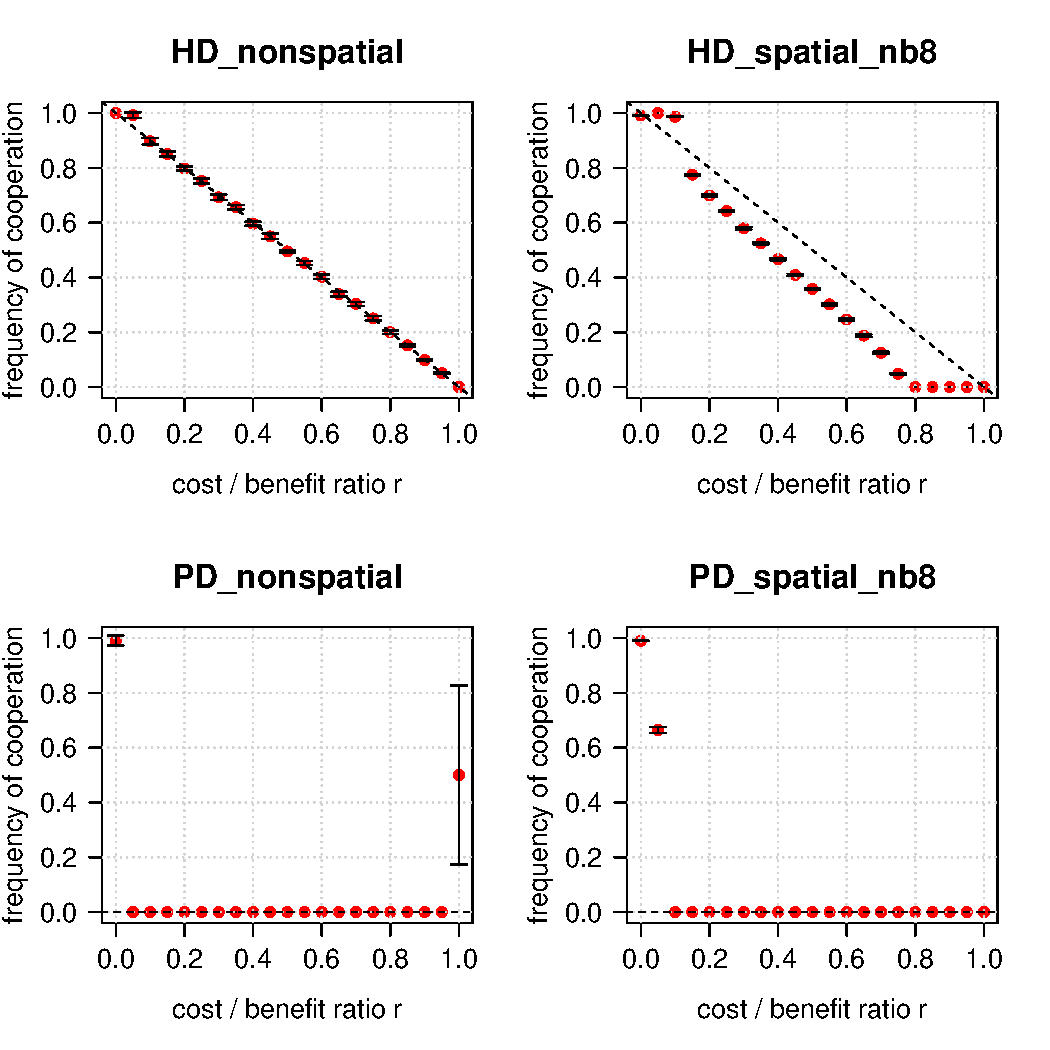
\includegraphics[width=9.5cm]{task1_4plot}
	\caption{Comparison of HD and PD game simulations, both with and without spatial structure.  \textbf{[ t = 5000, i = 10 ]} }\label{fig: task1_4plot}
\end{figure}






\subsection{Effect of neighbourhood size}


\textbf{HD games}[H] 

\begin{figure}
	\centering 
	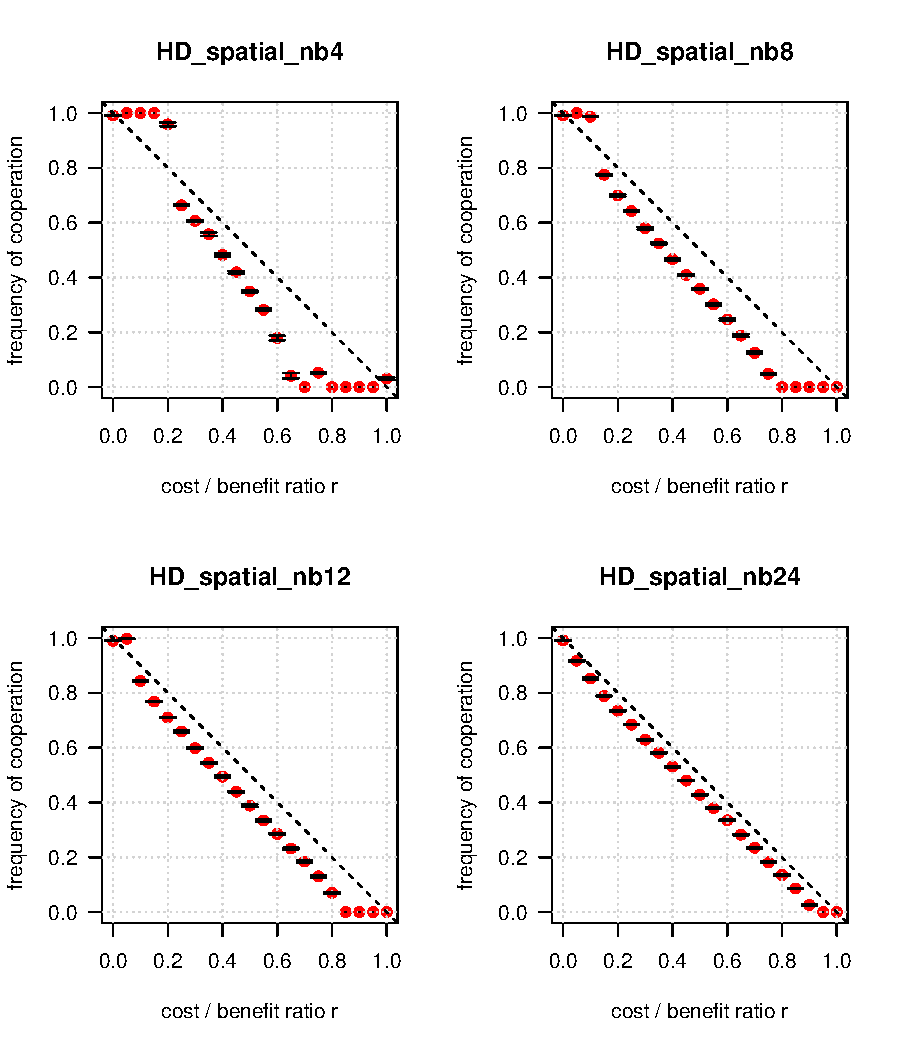
\includegraphics[width=9.5cm]{task2_4plot}
	\caption{Effect of varying neighborhood size in the HD game.  \textbf{[ t = 5000, i = 10 ]} }\label{fig: task2_4plot}
\end{figure}



\textbf{PD games} 


\begin{figure}[H]
	\centering 
	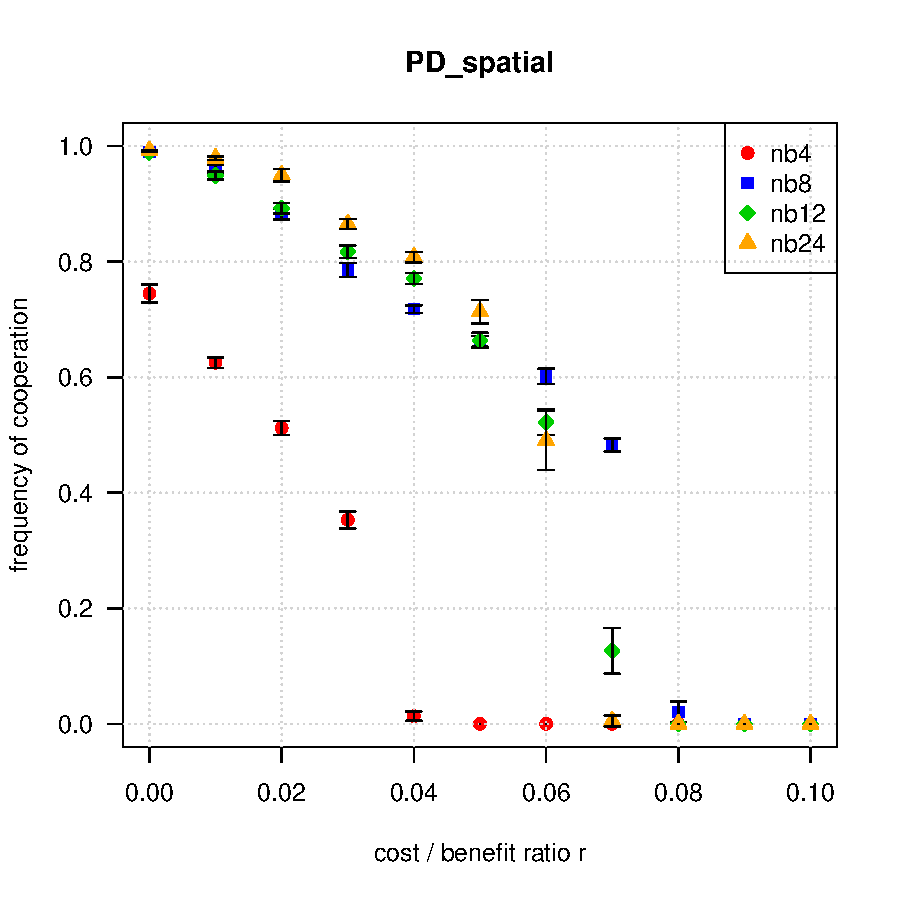
\includegraphics[width=9.5cm]{task2_multiplot}
	\caption{Spatial PD game simulations with different neighbourhood sizes.  \textbf{[ t = 5000, i = 10 ]} }\label{fig: task2_multiplot}
\end{figure}





\subsection{Effect of mixed strategies}

